\documentclass[11pt, a4paper]{article}
\usepackage{pdfpages}
\usepackage{parallel}
\usepackage[T2A]{fontenc}
\usepackage{ucs}
\usepackage[utf8x]{inputenc}
\usepackage[polish,english,russian]{babel}
\usepackage{hyperref}
\usepackage{rotating}
\usepackage[inner=2cm,top=1.8cm,outer=2cm,bottom=2.3cm,nohead]{geometry}
\usepackage{listings}
\usepackage{graphicx}
\usepackage{wrapfig}
\usepackage{longtable}
\usepackage{indentfirst}
\usepackage{array}
\usepackage{tikzsymbols}
\usepackage{soul}
\usepackage[ruled,vlined]{algorithm2e}
%\counterwithout{figure}{section} 

\usepackage{url}
\makeatletter
\g@addto@macro{\UrlBreaks}{\UrlOrds}
\makeatother

\newcolumntype{P}[1]{>{\raggedright\arraybackslash}p{#1}}
\frenchspacing
\usepackage{fixltx2e} %text sub- and superscripts
\usepackage{icomma} % коскі ў матэматычным рэжыме
\PreloadUnicodePage{4}

\newcommand{\longpage}{\enlargethispage{\baselineskip}}
\newcommand{\shortpage}{\enlargethispage{-\baselineskip}}

\def\switchlang#1{\expandafter\csname switchlang#1\endcsname}
\def\switchlangbe{
\let\saverefname=\refname%
\def\refname{Літаратура}%
\def\figurename{Іл.}%
}
\def\switchlangen{
\let\saverefname=\refname%
\def\refname{References}%
\def\figurename{Fig.}%
}
\def\switchlangru{
\let\saverefname=\refname%
\let\savefigurename=\figurename%
\def\refname{Литература}%
\def\figurename{Рис.}%
}

\hyphenation{admi-ni-stra-tive}
\hyphenation{ex-pe-ri-ence}
\hyphenation{fle-xi-bi-li-ty}
\hyphenation{Py-thon}
\hyphenation{ma-the-ma-ti-cal}
\hyphenation{re-ported}
\hyphenation{imp-le-menta-tions}
\hyphenation{pro-vides}
\hyphenation{en-gi-neering}
\hyphenation{com-pa-ti-bi-li-ty}
\hyphenation{im-pos-sible}
\hyphenation{desk-top}
\hyphenation{elec-tro-nic}
\hyphenation{com-pa-ny}
\hyphenation{de-ve-lop-ment}
\hyphenation{de-ve-loping}
\hyphenation{de-ve-lop}
\hyphenation{da-ta-ba-se}
\hyphenation{plat-forms}
\hyphenation{or-ga-ni-za-tion}
\hyphenation{pro-gramming}
\hyphenation{in-stru-ments}
\hyphenation{Li-nux}
\hyphenation{sour-ce}
\hyphenation{en-vi-ron-ment}
\hyphenation{Te-le-pathy}
\hyphenation{Li-nux-ov-ka}
\hyphenation{Open-BSD}
\hyphenation{Free-BSD}
\hyphenation{men-ti-on-ed}
\hyphenation{app-li-ca-tion}

\def\progref!#1!{\texttt{#1}}
\renewcommand{\arraystretch}{2} %Іначай формулы ў матрыцы зліпаюцца з лініямі
\usepackage{array}

\def\interview #1 (#2), #3, #4, #5\par{

\section[#1, #3, #4]{#1 -- #3, #4}
\def\qname{LVEE}
\def\aname{#1}
\def\q ##1\par{{\noindent \bf \qname: ##1 }\par}
\def\a{{\noindent \bf \aname: } \def\qname{L}\def\aname{#2}}
}

\def\interview* #1 (#2), #3, #4, #5\par{

\section*{#1\\{\small\rm #3, #4. #5}}
\ifx\ParallelWhichBox\undefined%
    \addcontentsline{toc}{section}{#1, #3, #4}%
\else%
\ifnum\ParallelWhichBox=0%
    \addcontentsline{toc}{section}{#1, #3, #4}%
\fi\fi%

\def\qname{LVEE}
\def\aname{#1}
\def\q ##1\par{{\noindent \bf \qname: ##1 }\par}
\def\a{{\noindent \bf \aname: } \def\qname{L}\def\aname{#2}}
}

\newcommand{\interviewfooter}[1]{
\vskip 1em
\noindent \textit{#1}
}

\switchlang{en}
\begin{document}

\title{2000 "--- SurfMouse mouse}
\date{}
\maketitle
\selectlanguage{english}
The SurfMouse is a typical example of a skeuomorph -- a device that imitates the appearance of another object that has nothing to do with its main function. It is easy to see that in this case the appearance of a surfboard is copied (fig. \ref{fig:SurfMousePic}).

\begin{figure}[h]
    \centering
    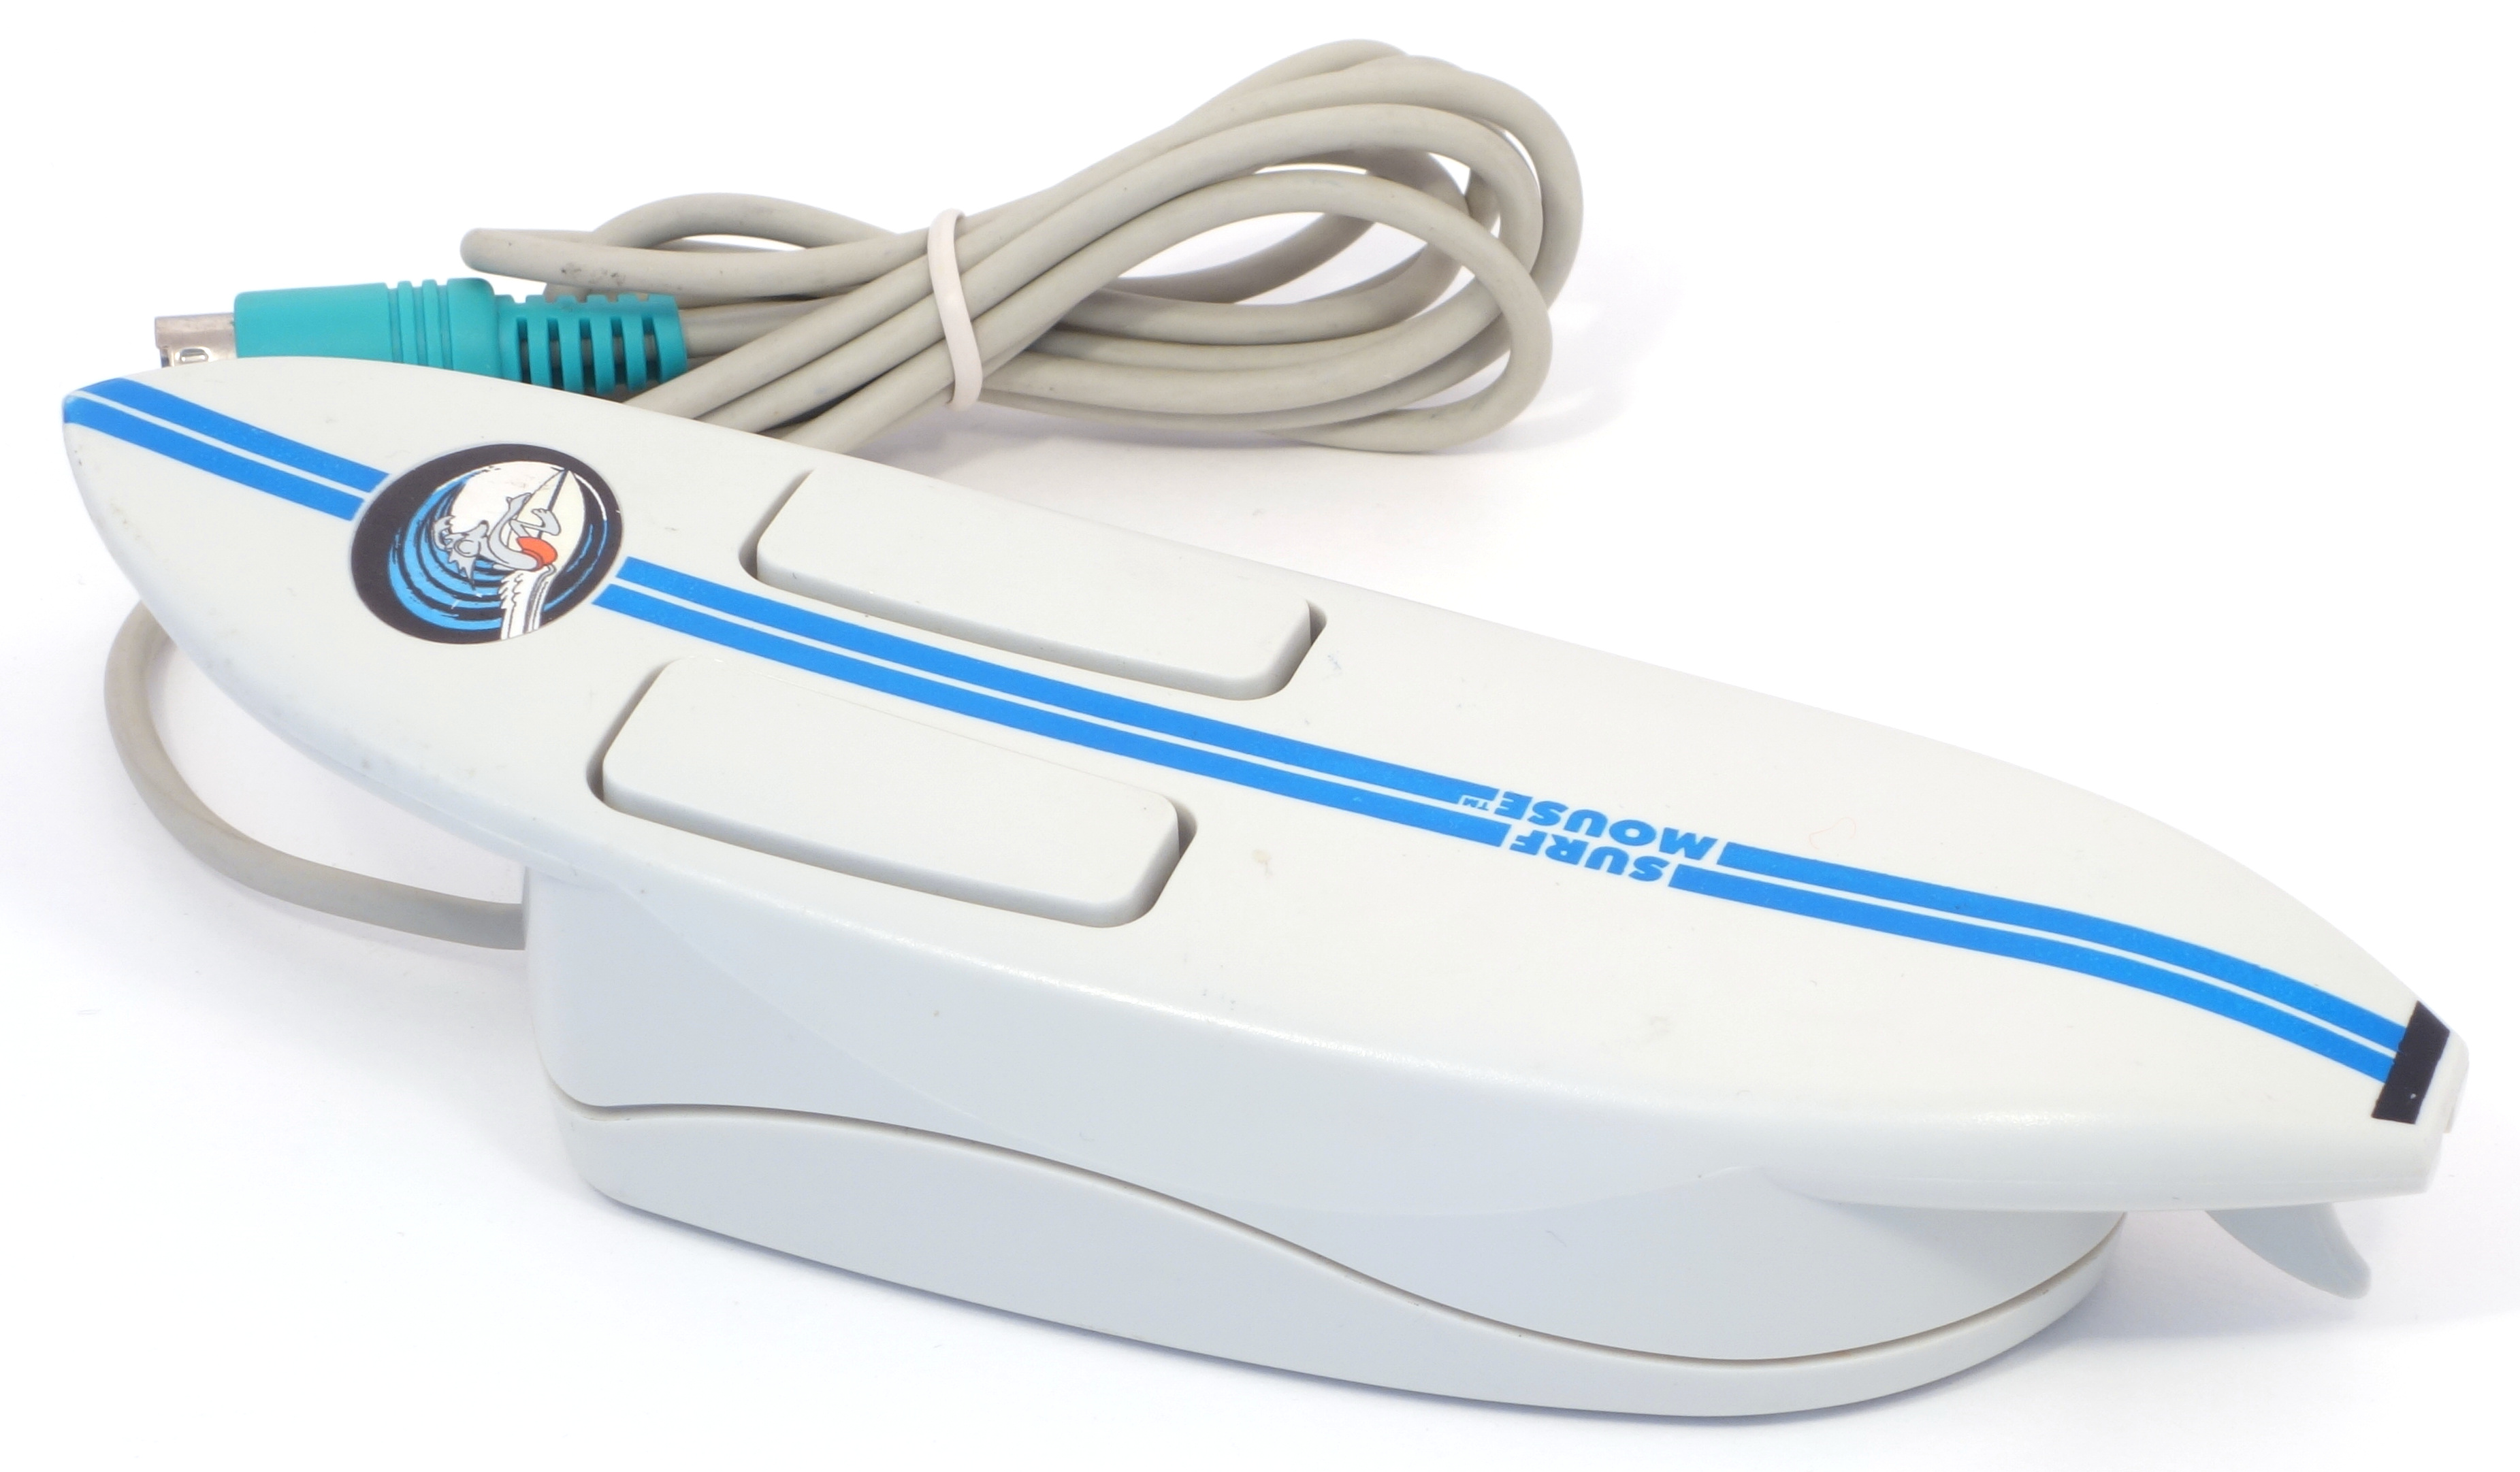
\includegraphics[scale=0.4]{2000_surf_mouse/pic_60.jpg}
    \caption{SurfMouse mouse}
    \label{fig:SurfMousePic}
\end{figure}

The mouse has a symmetrical body, the upper part of which is shaped like a surfboard. Because of this, it protrudes significantly back and forth, hanging over the main part, which retains the shape of a typical optomechanical mouse (fig. \ref{fig:SurfMouseTopBottom}). On the upper side of the case there are ornamental elements with the SurfMouse logo, as well as two large buttons. The buttons are located closer to the center than to the front of the case (in fact, they occupy the usual position for mice, and their visible shift to the center is caused solely by the protruding nose of the surfboard).

\begin{figure}[h]
    \centering
    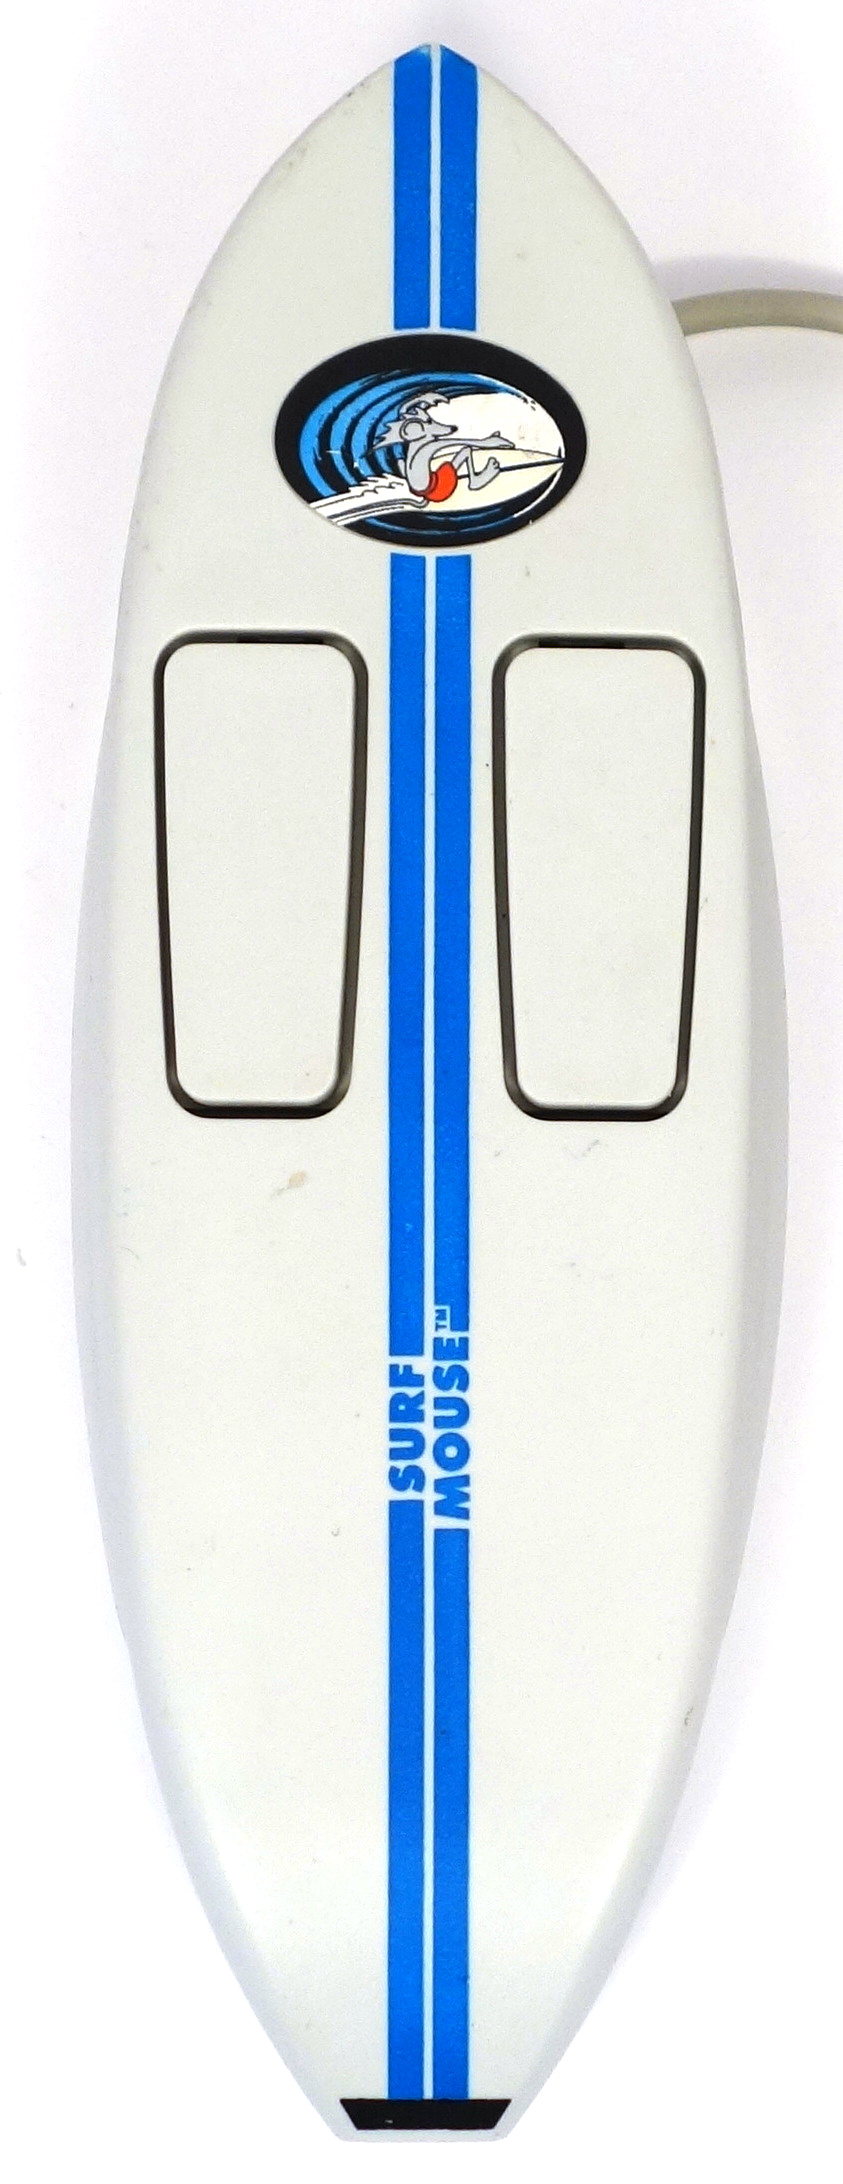
\includegraphics[scale=0.46]{2000_surf_mouse/top_60.jpg}
    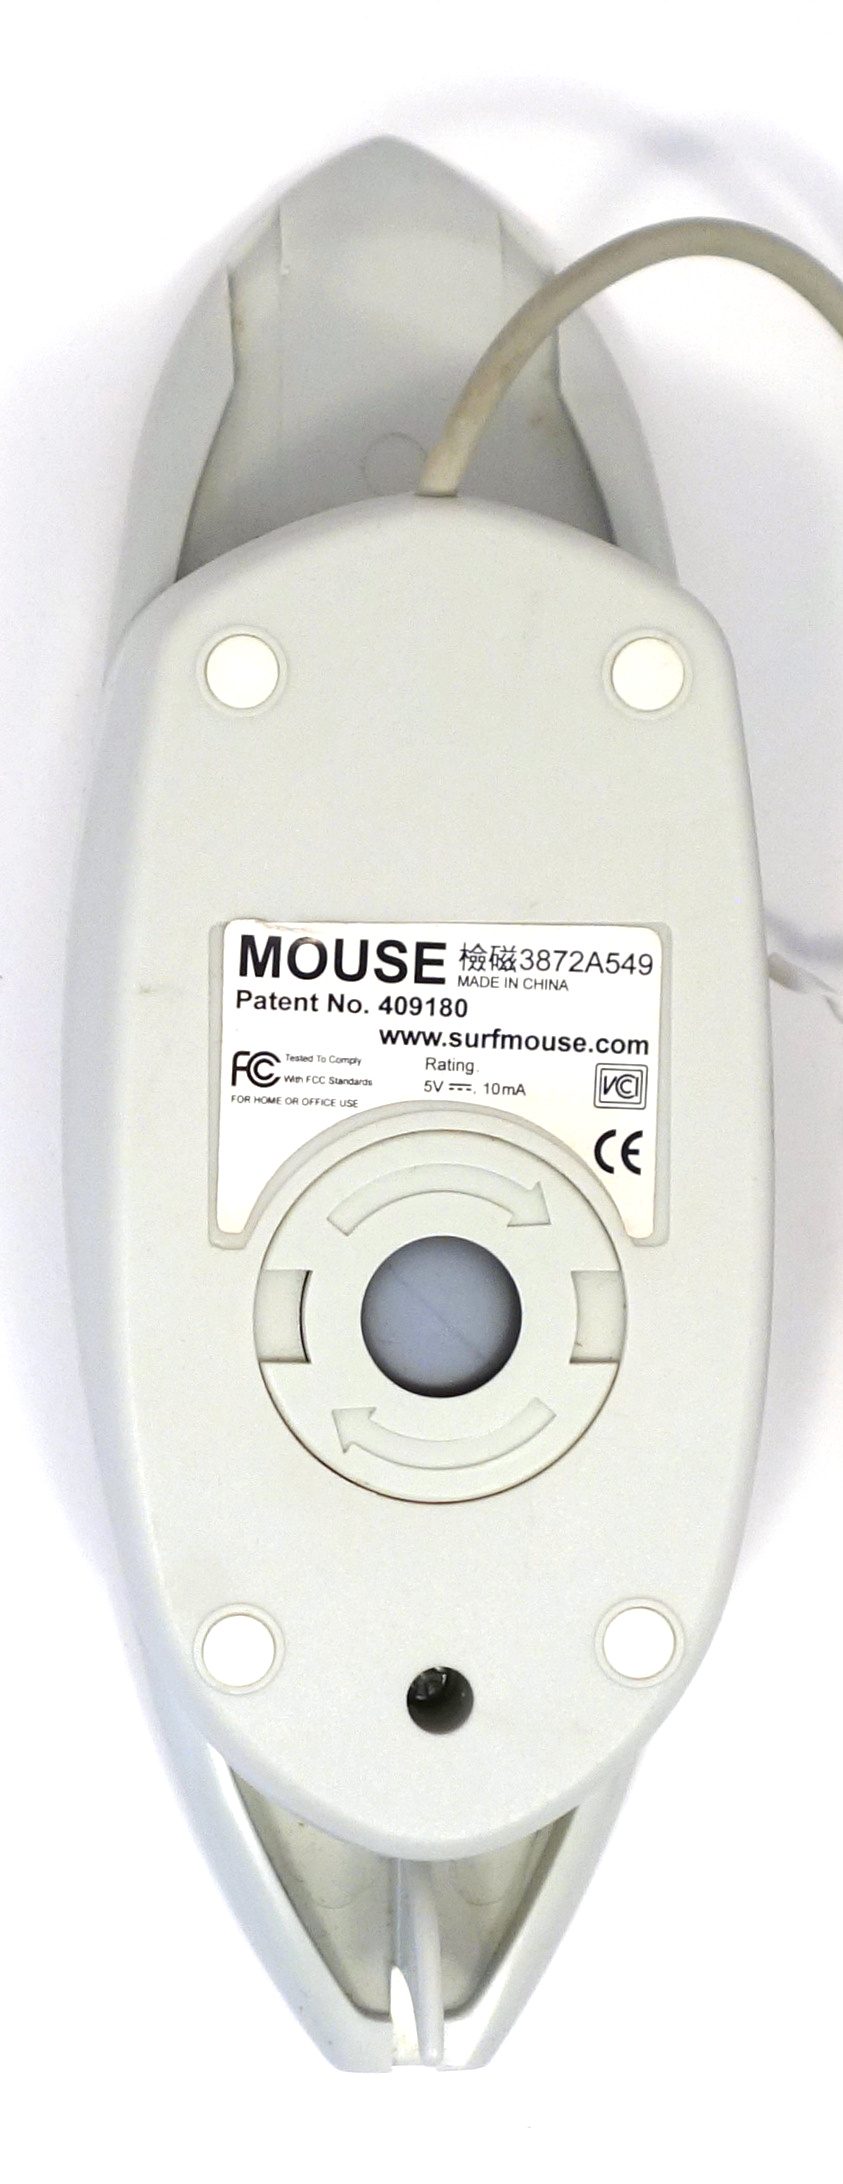
\includegraphics[scale=0.46]{2000_surf_mouse/bottom_60.jpg}
    \caption{SurfMouse mouse, top and bottom views}
    \label{fig:SurfMouseTopBottom}
\end{figure}

Turning the mouse over reveals a traditional 90s mouse ring that covers a rubber ball, low friction polymer sliding feet, and a sticker with some text.

Due to the need to copy the shape of the board, the mouse is larger than typical manipulators (fig. \ref{fig:SurfMouseSize}) thanks to the elongated front and back.

\begin{figure}[h]
    \centering
    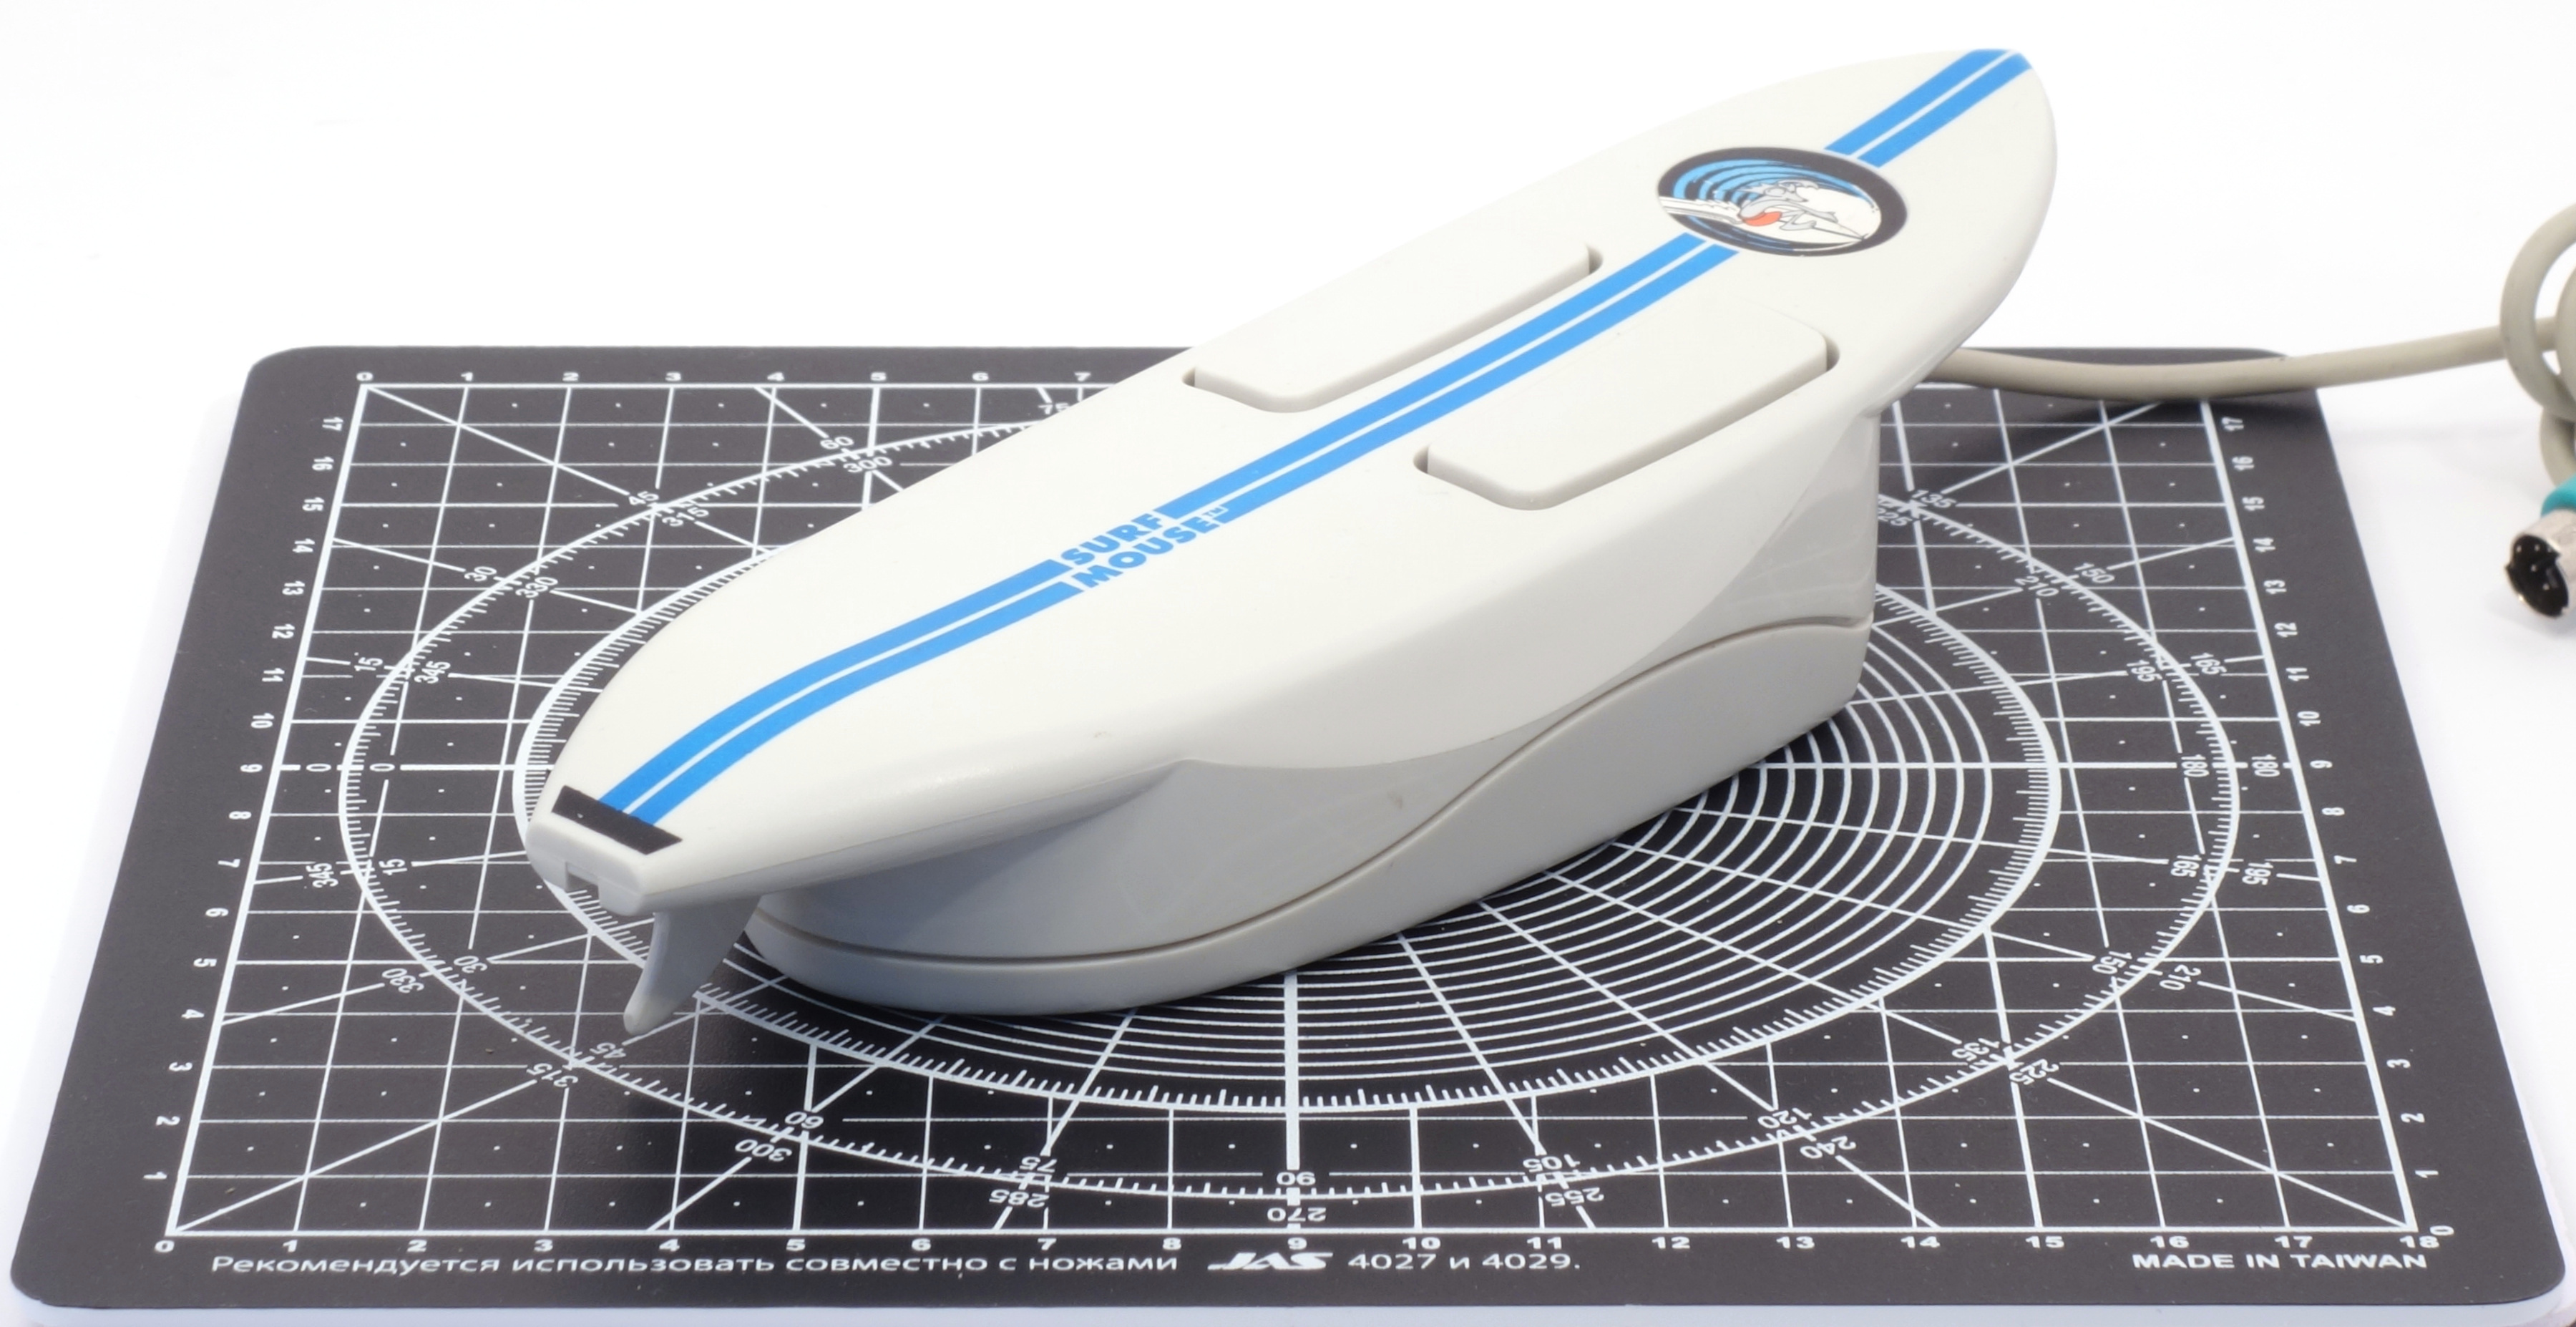
\includegraphics[scale=0.5]{2000_surf_mouse/size_30.jpg}
    \caption{SurfMouse mouse on a graduated pad with a grid step of 1~cm}
    \label{fig:SurfMouseSize}
\end{figure}

Due to the symmetry, the mouse is equally suitable for both left-handers and right-handers. In general, the hand lies on the mouse quite comfortably (fig. \ref{fig:SurfMouseHand}). The ``surfboard'' part closest to the user is bent down, forming a convenient horizontal wrist rest, and the position of the buttons and their shape can also be considered usable.

\begin{figure}[h]
    \centering
    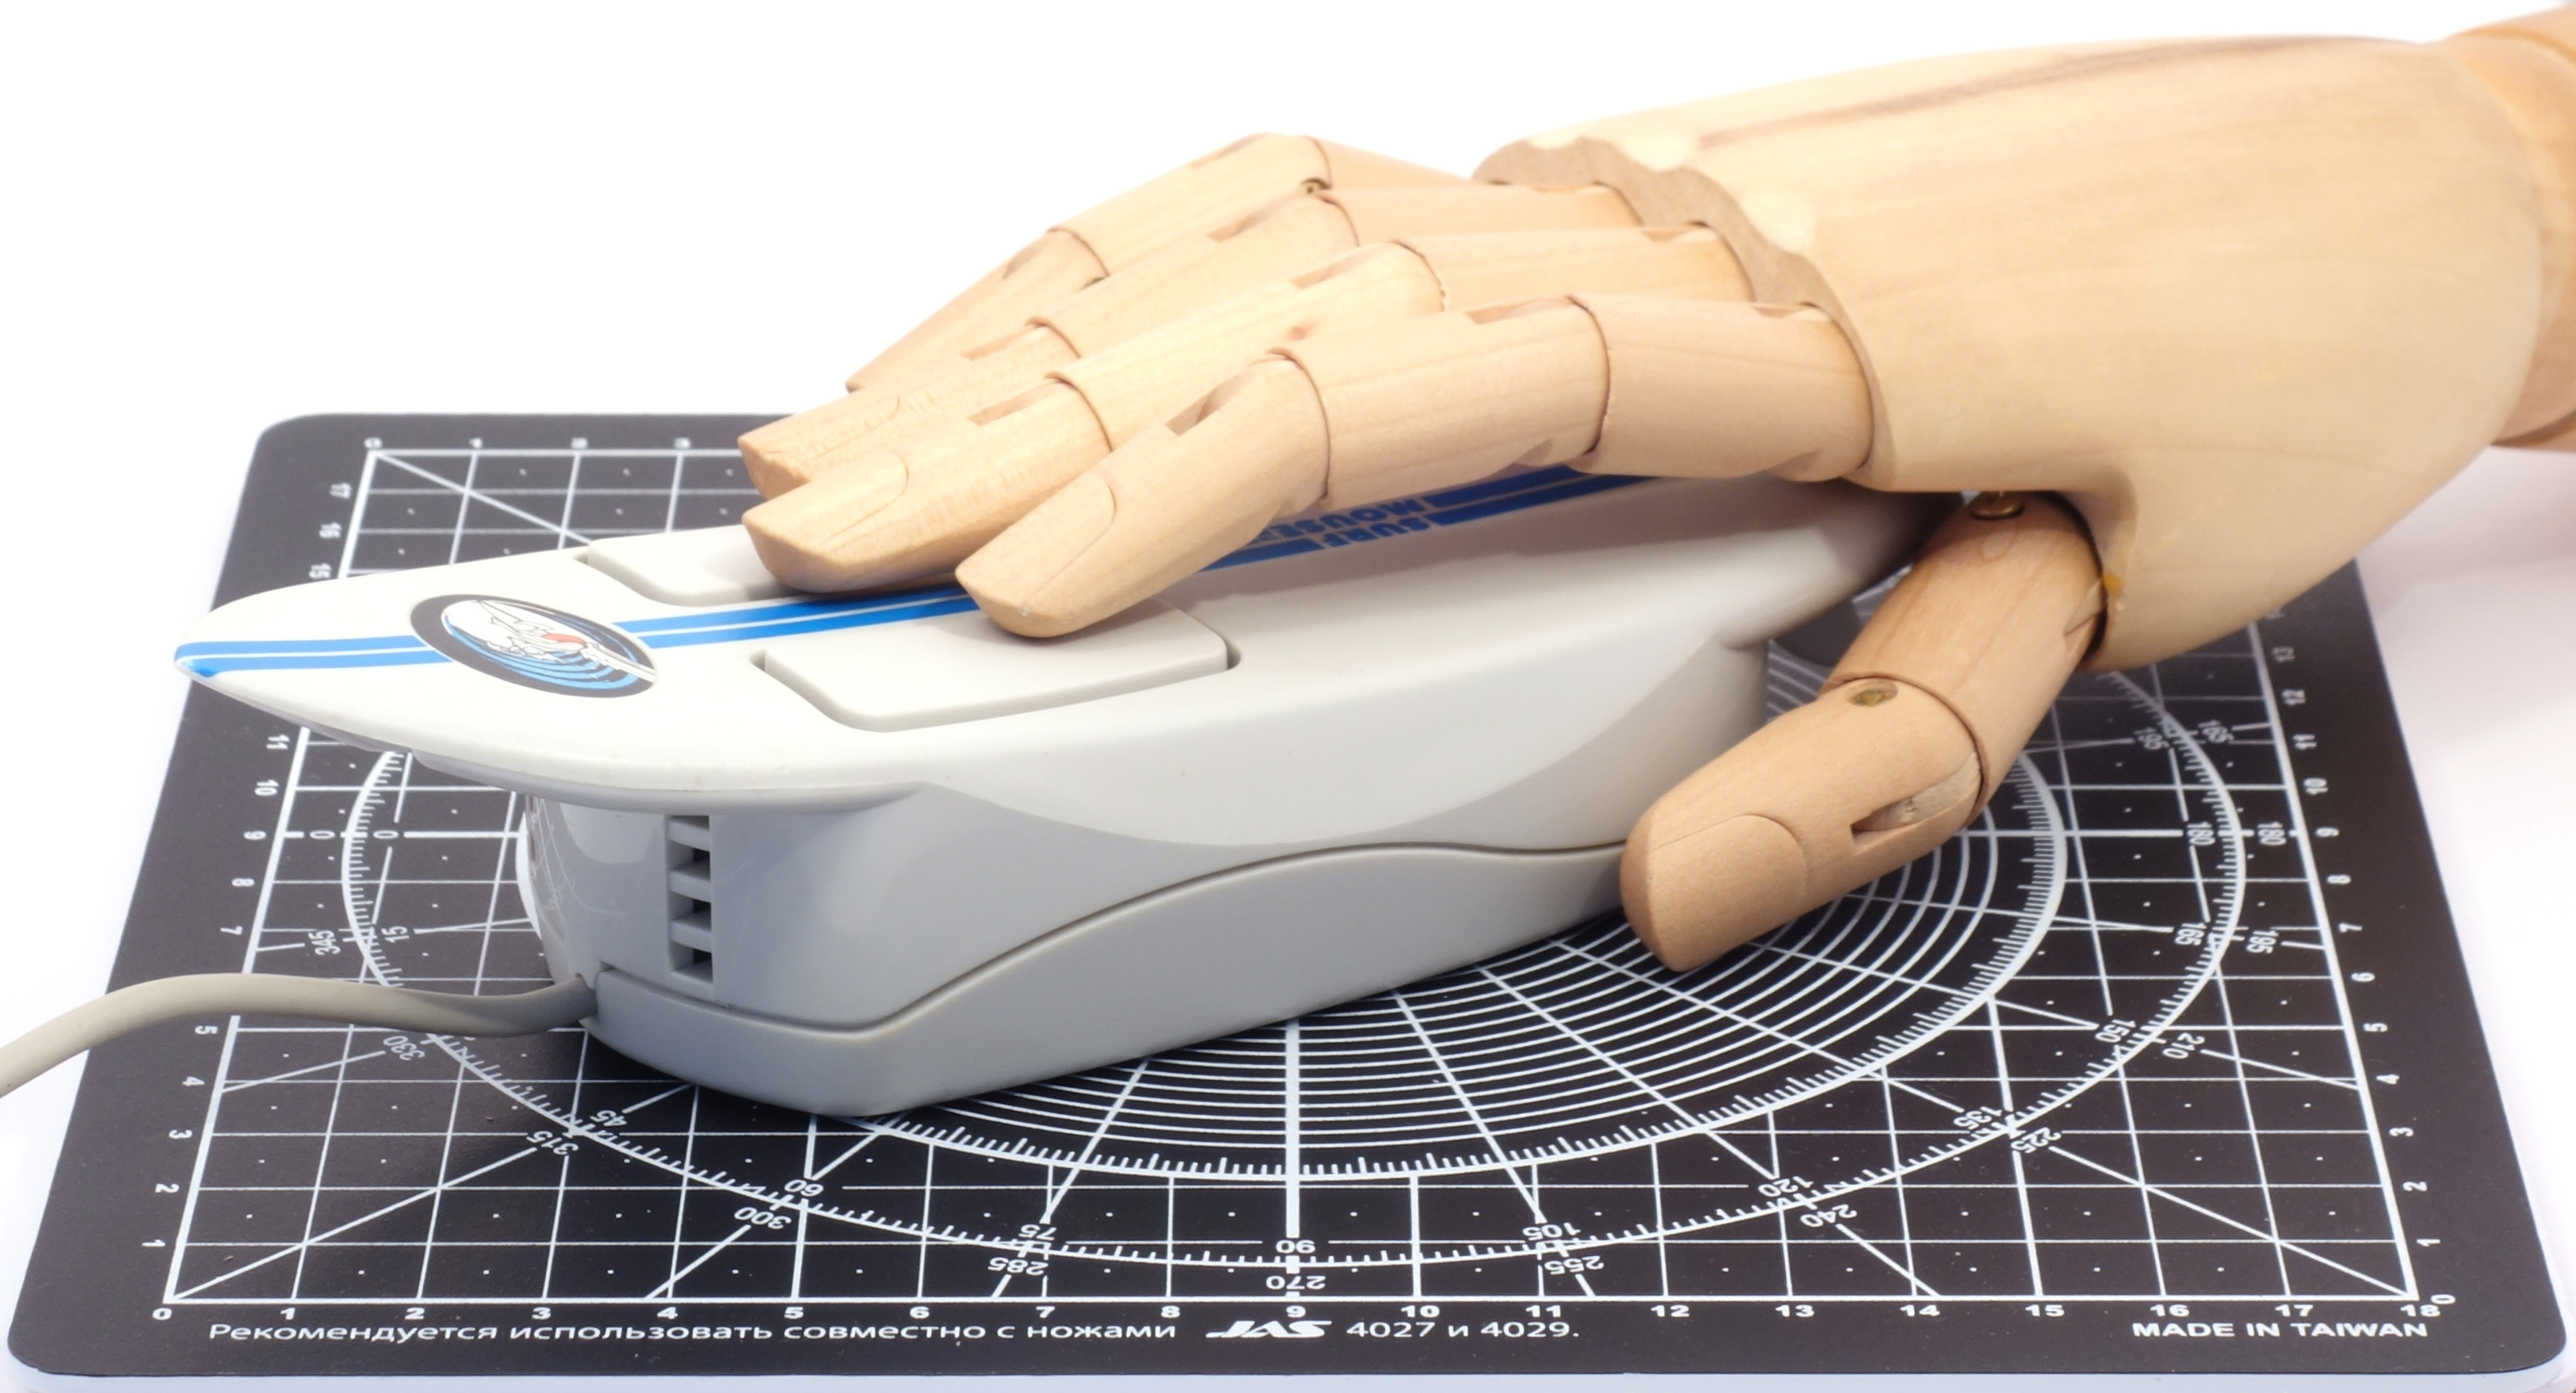
\includegraphics[scale=0.5]{2000_surf_mouse/hand_30.jpg}
    \caption{SurfMouse mouse with a human hand model}
    \label{fig:SurfMouseHand}
\end{figure}

Obviously, the developers relied on good ergonomics due to the comfortable position of the hand on the surfboard (they created a separate website \url{surfmouse.com} \cite{site} specifically for this mouse). However, the lack of a scroll wheel, which did not fit the style of a surfboard, was already a critical flaw in mouse ergonomics in 2000.

\begin{figure}[h]
    \centering
    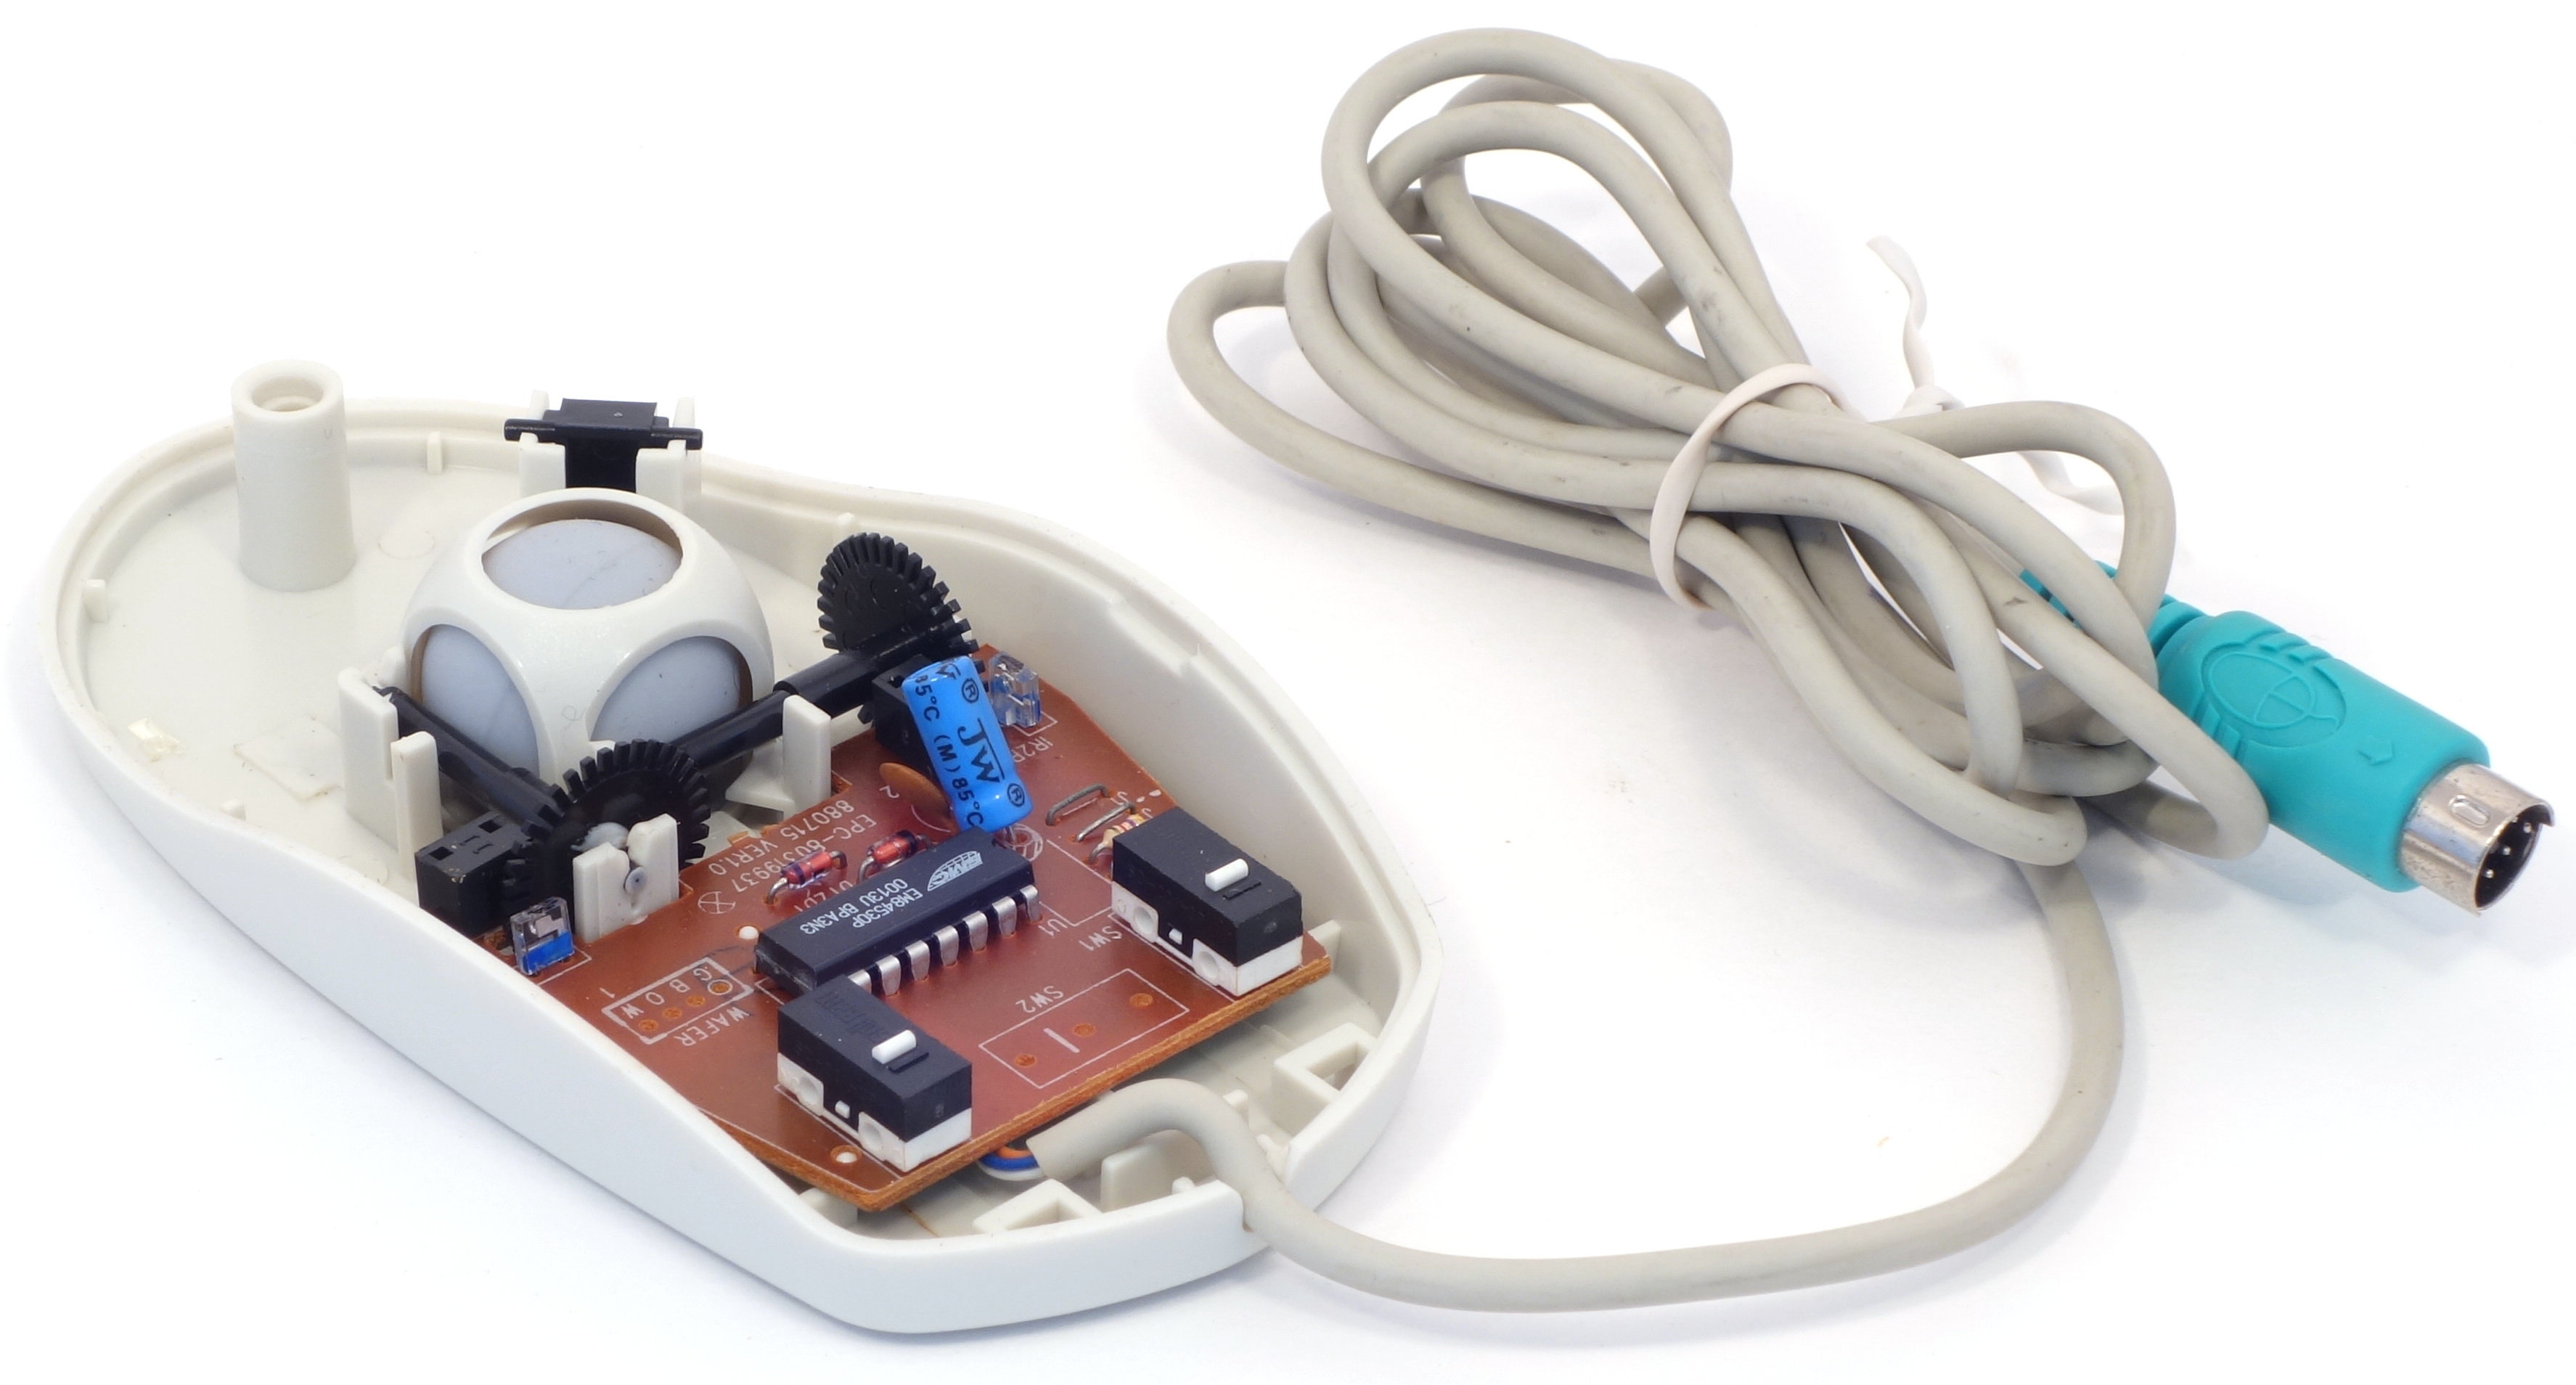
\includegraphics[scale=0.6]{2000_surf_mouse/inside_60.jpg}
    \caption{SurfMouse mouse disassembled}
    \label{fig:SurfMouseInside}
\end{figure}

The insides of this manipulator, shown in fig. \ref{fig:SurfMouseInside}, reveals a typical optomechanical design from the first half or mid-nineties. Moreover, it seems quite probable that there was a donor mouse in the 90s, the lower part and filling of which served as the basis for SurfMouse.

\begin{thebibliography}{9}
    \bibitem {site} Welcome to SurfMouse.com -- Surf the Web in Style! \url{https://web.archive.org/web/20001204212200/http://www.surfmouse.com/}
\end{thebibliography}

\end{document}
